\documentclass[a4paper, 12pt]{article} % Here we specify the paper size, font size and document type

\usepackage{cmap} % Make pdf searchable
\usepackage[T2A]{fontenc} % 
\usepackage[utf8]{inputenc} % encoding on source document
\usepackage[english, russian]{babel} % Multi language supporting
\usepackage{graphicx} % This package allows working with images
\usepackage{mathtools} % This package need to working with math
\usepackage{amsfonts}
\usepackage{amsmath} % This package is needed in order to set numbers only for those formulas that are referenced in the text
\usepackage{amssymb}
\usepackage{indentfirst}
\usepackage{pgfplots}
\usepackage{listings}

\newcommand{\retainlabel}[1]{\label{#1}\sbox0{\ref{#1}}}

\usepackage[backend=biber]{biblatex}
\addbibresource{lib.bib}


\usepackage[left=2cm,right=2cm,
    top=2cm,bottom=2cm,bindingoffset=0cm]{geometry}

\begin{document}

\section*{Предел числовой \cite{zorich}последовательности}
Определение. Число A $\in \mathbb{R}$ называется пределом числовой последовательности $\{x_n\}$, если для любой окресности V(A) точки A существует такой номер N (выбираемый в зависимости от V(A)), что все члены последовательности, номера которых больше N, содержатся в указанной окрестности точки A.


\begin{equation}
    (\lim_{n\to\infty} x_{n} = A) := \forall V(A) \exists N \in \mathbb{N} \forall n > N (x_n \in V(A))
\end{equation}

и соответственно

\begin{equation}
    (\lim_{n \to \infty} x_{n} = A) := \forall \varepsilon > 0 \ \exists N \in \mathbb{N} \ \forall n > N \ (|x_n - A| < \varepsilon).
\end{equation}

\clearpage

\section*{Предел функции}
Определение. Итак, число A называется пределом функции $f: E \to \mathbb{R}$ при $x$, стемящемся по множеству $E$ к точке $a$ (предельной для $E$), если для любой окрестности точки $A$ найдется проколотая окрестность точки $a$ в множестве $E$, образ которой при отображении $f : E -> \mathbb{R}$ содержится в заданной окрестности точки $A$.

\begin{equation}
    (\lim_{E \ni x \to a} f(x) = A) := \forall V_\mathbb{R}(A) \ \exists \dot{U}_E(a) \ (f(\dot{U}_E(a)) \subset V_\mathbb{R}(A))
\end{equation}

\clearpage
\section*{Замечательные пределы}

Первый замечательный предел:

\begin{equation}
    \lim_{n \to 0} \frac{\sin x}{x} = 1
\end{equation}

Второй замечательный предел:

\begin{equation}
    \lim _{{x\to \infty }}\left(1+{\frac  {1}{x}}\right)^{x}=e.
\end{equation}

\clearpage


\section*{Разложение фукнции в ряд Тейлора}

\begin{equation}
    P_n(x_0; x) = P_n(x) = f(x_0) + \frac{f'(x_0)}{1!}(x - x_0) + ... + \frac{f^{(n)}(x_0)}{n!}(x - x_0)^n
    \label{eq:dec_to_Teylor}
\end{equation}

Определение. Алгебраический полином, заданный соотношением (\ref{eq:dec_to_Teylor}), называется полиномом Тейлора\footnote{Б. Тейлор (1685 - 1731) -- английский математик} порядка $n$ функции $f(x)$ в точке $x_0$.

Нас будет интересовать величина
\begin{equation}
    f(x) - P_n(x_0; x) = r_n(x_0; x)
\end{equation}
уклонение полинома $P_n(x)$ от функции $f(x)$, называется часто остатком, точнее, $n$-м остатком или $n$-м остаточным членом формулы Тейлора:

\begin{equation}
    f(x) = f(x_0) + \frac{f'(x_0)}{1!} (x - x_0) + ... + \frac{f^{(n)}(x_0)}{n!} (x - x_0)^n + r_n (x_0; x)
    \label{eq:for_of_Teylor}
\end{equation}

Также давайте разложим наиболее часто используемые функции по формуле (\ref{eq:for_of_Teylor}):
\begin{equation}
    e^x = 1 + \frac{1}{1!}x + \frac{1}{2!}x^2 + \frac{1}{3!}x^3 + ... + \frac{1}{n!}x^n + O(x^n + 1)
\end{equation}
\begin{equation}
    \cos x = 1 - \frac{1}{2!}x^2 + \frac{1}{4!}x^4 - \frac{1}{6!}x^6 + ... + \frac{(-1)^k}{2k!}x^{2k} + O(x^{2k+2})
\end{equation}

\begin{equation}
    \sin x = x - \frac{1}{3!}x^3 + \frac{1}{5!}x^5 - \frac{1}{7!}x^7 + ... + \frac{(-1)^k}{(2k + 1)!}x^{2k + 1} + O(x^{2k+3})
\end{equation}

\begin{equation}
    \ln(1 + x) = x - \frac{1}{2}x^2 + \frac{1}{3}x^3 - \frac{1}{4}x^4 + ... + \frac{(-1)^{n - 1}}{n}x^n + O(x^{n + 1})
\end{equation}

\clearpage

\section*{Интеграл Римана}

Определение. Функция $f$ называется интегрируемой по Риману на отрезке $[a, b]$, если для нее существует указанный в пункте (\ref{eq:int_Riman}) предел интегральных сумм при $\lambda (P) \to 0$ (т.е. если для нее определен интеграл Римана).

Множество всех функций, интегрируемых по Риману на отрезке $[a, b]$, будет обозначаться через $\Re [a, b]$.

\[
    \int^b_a f(x) dx := \lim_{\lambda(P) \to 0} \sum^n_{i = 1} f(\xi_i) \Delta x_i
    \label{eq:int_Riman}
\]

\clearpage

\section*{Формула Тейлора}

Теорема. Если функция $f: U(x) \to \mathbb{R}$ определена и принадлежит классу $C^{(n)} \ (U(x); \mathbb{R})$ в окрестности $U(x) \subset \mathbb{R}^m$, а отрезок $[x, x + h]$ полностью содержится в $U(x)$, то имеет место равенство

\begin{eqnarray*}
    f(x^1 + h^1, ..., x^m+h^m) - f(x^1, ...,x^m) = \\ = \sum^{n - 1}{k = 1} \frac{1}{k!} (h^1 \delta_1 + ... + h^m \delta_m)^k f(x) + r_{n - 1}(x; h),
\end{eqnarray*}
где
\begin{equation}
    r_{n-1}(x;h) = \int^1_0 \frac{(1-t)^{n - 1}}{(n - 1)!} (h^1 \delta_1 + ... + h^m \delta_m)^n f(x + th) dt
\end{equation}

\clearpage
\section*{Интеграл по гладкой поверхности}
Определение. (интеграла от $k$-формы $\omega$ по заданной картой $\varphi: I \to S$ гладкой $k$-мерной поверхности).

\[
    \int_S \omega := \lim_{\lambda (P) \to 0} \sum_i \omega (x_i)(\varepsilon_1, ..., \varepsilon_k) = \lim_{\lambda \to 01} \sum_i (\varphi * \omega)(\tau_i)(\tau_1, ..., \tau_k).
    \label{eq:int_by_smooth_surface_one}
\]

Если применить это определение к $k$-форме $f(t) dt^1 \land ...\land dt^k$ на $I$ (когда $\varphi$ -- тождественное отображение), то очевидно, получим, что:

\[
    \int_I f(t) dt^1 \land ... \land dt^k = \int_I f(t) dt^1 ... \ dt^k.
    \label{eq:int_by_smooth_surface_two}
\]

Таким образом, из (\ref{eq:int_by_smooth_surface_one}) следует, что
\begin{equation}
    \int_{S = \varphi(I)} \omega = \int_I \varphi * \omega,
\end{equation}

а последний интеграл, как видно из равенства (\ref{eq:int_by_smooth_surface_two}), сводится к обычному кратному интегралу от соответствующей форме $\varphi * \omega$ функции $f$ на промежутке $I$.

\clearpage
\section*{Формула Стокса в $\mathbb{R}^3$}
Утверждение. Пусть S -- ориентированная кусочно гладкая компатная двумерная поверхность с краем $\delta S$, лежаща в области $G \subset \mathbb{R^3}$, в которой задана гладкая 1-форма $\omega = P\ dx + Q\ dy + R\ dz$. Тогда имеет место соотношение
\begin{eqnarray*}
    \int_{\delta S} P\ dx + Q\ dy + R\ dz = \iint_S \left( \frac{\delta R}{\delta y} - \frac{\delta Q}{\delta z} \right) \ dy \land dz + \\ + \left(\frac{\delta P}{\delta z} - \frac{\delta R}{\delta x}\right) dz \land dx + \left(\frac{\delta Q}{\delta x} - \frac{\delta P}{\delta y}\right) dx \land dy,
\end{eqnarray*}
где ориентация края $\delta S$ берется согласованной с ориентаией поверхности S.

\clearpage

\section*{Алгебра форм}
Пусть $X$ - линейное пространство, а $F^k : X^k \to \mathbb{R}$ -- вещественнозначная $k$-форма на $X$. Если $e_1, ..., e_n$ -- базис в $X$, а $x_1 = x^{i_1} e_{i_1}, ..., x_k = x^{i_k} e_{i_k}$ -- разложение векторов $x_1, ..., x_k \in X$ по этому базису, то в силу линейности $F_k$ по каждому аргументу

\begin{equation}
    F^k(x_1,...,x_k) = F^k(x^i_1 e_{i_1}, ..., x^i_k e_{i_k}) = F^k(e_{i_1}, ..., e_{i_k}) x^{i_1} \cdot  ... \cdot x^{i_k} = a_{i_1 ... i_k} x^{i_1} \cdot x^{i_k}.
\end{equation}

\clearpage
\section*{График функции $f(x) = \sin \frac{1}{x} $}
\begin{center}
    \begin{tikzpicture}
        \begin{axis}[
                axis lines=middle,
                ticklabel style={fill=white},
                width=15cm, height=8cm,
                xmin=-1.2,xmax=1.2,
                ymin=-1.5,ymax=1.5,,
                xlabel=$x$,ylabel=$y$,
            ]
            \addplot[blue,samples=50,domain=-1:-0.2,smooth] {sin(1/\x r)};
            \addplot[blue,samples=1000,domain=-0.2:-0.02]   {sin(1/\x r)};
            \addplot[blue,samples=1000,domain=0.02: 0.20]   {sin(1/\x r)};
            \addplot[blue,samples=50,domain= 0.2: 1,smooth] {sin(1/\x r)};
        \end{axis}
    \end{tikzpicture}
\end{center}

\clearpage
\section*{Аксиоматика и некоторые общие свойства множества действительных чисел}

Определение. Множество $\mathbb{R}$ называется множеством действительных (вещественных) чисел, а его элементы -- действительными (вещественными) числами, если выполнен следующий комплекс условий, называемый аксиоматикой вещественных чисел:

\begin{enumerate}
    \item [(I)] Аксиомы сложения. Определено отображение (операции сложения)
          $$ + : \mathbb{R} \times \mathbb{R} \to \mathbb{R} $$
          сопоставляющее каждой упорядоченной паре $(x, y)$ элементов $x, y$ из $\mathbb{R}$ некоторый элемент $x+y \in \mathbb{R}$, называемый суммой $x$ и $y$. При этом выполнены следующие условия:
          \begin{enumerate}
              \item [$1_+.$] Существует нейтральный элемент 0 (называемый в случае сложения нулем):
                    $$ \exists 0 \ \forall x: x + 0 = x. $$
              \item [$2_+.$] Для любого элемента $x \in \mathbb{R}$ имеется элемент $-x \in \mathbb{R}$, называемый противоположным к $x$, такой, что
                    $$ x + (-x) = (-x) + x = 0. $$
              \item [$3_+.$] Операция + ассоциативна, т.е. для любых элементов $x, y, z \in \mathbb{R}$ выполнено $$ x + (y + z) = (x + y) + z. $$
              \item [$4_+.$] Операция + коммутативна, т.е. для любых элементов $x, y \in \mathbb{R}$ выполнено $$ x + y = y + z $$
          \end{enumerate}
    \item [(II)] Аксиомы умножения. Определено отражение (операция умножения) $$ \bullet : \mathbb{R} \times \mathbb{R} \to \mathbb{R}, $$ сопоставляющее каждой упорядоченной паре $(x, y)$ элементов $x, y \in \mathbb{R}$ некоторый элемент $x \cdot y \in \mathbb{R}$, называемый произведением $x$ и $y$, причем так, что выполнены следующие условия:
          \begin{enumerate}
              \item [$1_\bullet.$] Существует нейтральный элемент $1 \in \mathbb{R} \backslash 0$ (называемый в случае умножения единицей) такой, что $$ \exists 1 \ \forall x: x \cdot 1 = x.$$
              \item [$2_\bullet.$] Для любого элемента $x \in \mathbb{R} \backslash 0$ имеется элемент $x^-1 \in \mathbb{R}$, называемый обратным, такой, что $$ x \cdot x^-1 = x^-1 \cdot * x = 1.$$
              \item [$3_\bullet.$] Операция $\bullet$ ассоциативна, т.е. для любых $x, y, z \in \mathbb{R}$ $$ x \cdot (y \cdot z) = (x \cdot y) \cdot z.$$
              \item [$4_\bullet.$] Операция $\bullet$ коммутативна, т.е. для любых $x, y \in \mathbb{R}$ $$ x \cdot y = y \cdot x.$$
                    Заметим, что по отношению к операции умножения множество $\mathbb{R} \backslash 0$, как можно проверить, является (мультипликативной) группой.
          \end{enumerate}
\end{enumerate}

\clearpage

\section*{Умножение матриц}
Теорема 1. Произведение $\varphi A \varphi B$ двух линейных отображений с матрицами $A$ и $B$ является линейным отображением с матрицей $C = AB$. Другими словами
\begin{equation}
    \varphi A \varphi B = \varphi AB.
    \label{eq:mul_matrix}
\end{equation}
Мы можем забыть о линейных отображениях и находить произведение $AB$ двух произвольных матриц $A, B$, имея в виду, однако, что символ $AB$ имеет смысл только в том случае, когда число  столбцов в матрице $A$ совпадает с числом строк в матрице $B$. Именно при этом условии выполняется правило умножения $i-$й строки $A_{(i)}$ на $j-$й столбец $B^{(j)}$, согласно которому

\begin{equation}
    A_{(i)}B^{(j)} = (a_{i 1}, ..., a_{i s})[b_{1 j}, ..., b_{s j}]
    \label{eq:mult_matrix}
\end{equation}
Следствие. Умножение матриц ассоциативно:
\begin{equation}
    A(BC) = (AB)C
\end{equation}
Действительно, произведение матриц соответствует произведению линейных отображений (теорема 1 и соотношение \ref{eq:mul_matrix}). К тому же результату можно прийти вычислительным путём, используя непосредственно соотношение (\ref{eq:mult_matrix}). $\Box$

Обратим ещё внимание на так называемые законы дистрибутивности:
\begin{equation}
    (A + B)C = AC + BC, ~~~~~ D(A + B) = DA + DB
    \label{eq:distr_matrix}
\end{equation}
где $A, B, C, D$ -- произвольные матрицы размеров соответственно $m \times s, m \times s, s \times n, n \times m.$

Действительно, пологая $A = (a_{ij}), B = (b_{ij}), C = (c_{ij})$, мы получим для любых $i$, $j$ равенство (используя дистрибутивность в $\mathbb{R}$)
\begin{equation}
    \sum^n_{k = 1} (a_{ik} + b_{ik})c_{kj} = \sum^n_{k=1} a_{ik} c_{kj} + \sum^n_{k = 1} b_{ik} c_{kj},
\end{equation}
левая часть которого дает элемент $g_{ij}$ матрицы $(A + B)C$, а правая -- элементы $h_{ij}$ и $h'_{ij}$ матриц $AC$ и соответственно $BC$. Второй закон дистрибутивности (\ref{eq:distr_matrix}) проверяется совершенно аналогично.

\clearpage
\section*{Транспонирование матриц}
Будем говорить, что матрицы

\begin{equation}
    A =
    \begin{Vmatrix}
        a_{11} & a_{12} & ... & a_{1n} \\
        a_{21} & a_{22} & ... & a_{2n} \\
        \\
        a_{m1} & a_{m2} & ... & a_{mn}
    \end{Vmatrix},
    ~~~~~
    A^T =
    \begin{Vmatrix}
        a_{11} & a_{21} & ... & a_{m1} \\
        a_{12} & a_{22} & ... & a_{m2} \\
        \\
        a_{1n} & a_{2n} & ... & a_{mn}
    \end{Vmatrix}
\end{equation}
размеров $m \times n$ и $n \times m$ соответственно получаются друг из друга транспонированием -- заменой строк на столбцы, а столбцов на строки.

\clearpage
\section*{Инварианты линейных групп}
Линейной группой степени $n$ мы, как обычно, называем любую подгруппу в $GL(n, P)$, где $P$ -- некоторое поле. В дальнейшем можно считать $P = \mathbb{R}$ или $P = \mathbb{C}$. Если $G$ -- абстрактная группа и $\Phi : G \to GL(n, \mathbb{C})$ -- её линейное представление, то пару $(G, \Phi)$ мы тоже будем называть линейной группой. Линейные преобразования $\Phi_g$ действуют на столбцы переменных $x_1,...,x_n$:

\begin{equation}
    \begin{Vmatrix}
        \Phi_g(x_1) \\
        \vdots      \\
        \Phi_g(x_n)
    \end{Vmatrix}
    = \Phi_g
    \begin{Vmatrix}
        x_1    \\
        \vdots \\
        x_n.
    \end{Vmatrix}
\end{equation}
Они переводят любую форму (однородный многочлен) $f$ степени $m$ снова в форму степени $m$:
\begin{equation}
    (\widetilde{\Phi_g}f)(x_1, ..., x_n) = f(\Phi_{g^-1}(x1), ..., \Phi_{g^-1}(x_n)).
\end{equation}

Определение. Форма $f \in P_m$, остающаяся неподвижной при действии $\widetilde{\Phi_g}$ (т.е. $\widetilde{\Phi_g}f = f \ \forall g \in G$), называется (целым) инвариантом степени $m$ линейной группы $(G, \Phi)$.

\clearpage
\section*{Начала тензорного исчисления}
\textbf{1. Понятие то тензорах.} Разумной общности можно достичь, ограничившись лишь полилинейными отображениями некоторого специального вида.

Определение. Пусть $\Re$ -- поле, $V$ -- векторное пространство над $\Re, V^*$ -- сопряженное к $V$ пространство, $p$ и $q$ -- целые числа $\geq 0,$
\begin{equation}
    V^p \times (V^*)^q = \underbrace{V \times ... \times V}_{p} \times \underbrace{V^* \times V^*}_{q}
\end{equation}
-- декартово произведение $p$ экземпляров пространства $V$ и $q$ экземпляров пространства $V^*$. Всякое $(p + q)$ -- линейное отображение
\begin{equation}
    f: V^p \times (V^*)^q \to \Re
\end{equation}
называется тензором на $V$ типа $(p, q)$ и валентности (или ранга) $p + q$.

\textbf{2. Произведение тензоров.}Вначале пусть
\begin{equation}
    f: V_1 \times ... \times V_r \to \Re ~~~~~ g: W_1 \times ... \times W_s \to \Re
\end{equation}
-- произвольные полилинейные формы. Это значит, что $V_i, W_j$ -- никак не связанные друг с другом векторные пространства.

Определение. Под тензорным произведением $f$ и $g$ понимают отображение
\begin{equation}
    f \otimes g: V_1 \times ... V_r \times W_1 \times ... \times W_s \to \Re,
\end{equation}
определенное формулой
\begin{equation}
    (f \otimes g)(v_1, ..., v_r; w_1, ...., w_s) = f(v_1, ..., v_r)g(w_1, ..., w_s).
\end{equation}
Существенно подчеркнуть, что переменные $V_i$ независимы от переменных $W_j$.

Резюмируем сказанное:
\begin{enumerate}
    \item [$1_\otimes$] операция умножения $\otimes$ определена для тензоров произвольных типов;
    \item [$2_\otimes$] валентность произведения равна сумме валентностей сомножителей;
    \item [$3_\otimes$] тензорное произведение ассоциативно и дистрибутивно, но не коммутативно.
\end{enumerate}

\clearpage
\section*{Дифференциальное исчисление. Основные теоремы.}
Теорема. Пусть $f: U(x_0) \to \mathbb{R}$ -- функция класса $C^{(2)}(U(x_0); \mathbb{R})$, определенная в окрестности $U(x_0) \subset \mathbb{R}^m$ точки $x_0 = (x^1_0, ...,x^m_0) \in \mathbb{R}$, и пусть $x_0$ -- критическая точка этой функции $f$.

Если в тейлоровском разложении
\begin{equation}
    f(x^1_0+h^1, ..., x_0^m+h^m) = f(x_0^1, ..., x^m_0) + \frac{1}{2!} \sum^m_{i, j = 1} \frac{\delta^2 f}{\delta x^i \delta x^j} (x_0)h^i h^j + o(||h||^2)
    \label{eq:diff_expr_two}
\end{equation}
функции в точке $x_0$ квадратичная форма
\begin{equation}
    \sum_{i,j = 1}^m \frac{\delta^2 f}{\delta x^i \delta x^j} (x_0) h^i h^j \equiv \delta_{ij} f(x_0) h^i h^j
    \label{eq:diff_expr_one}
\end{equation}
\begin{enumerate}
    \item [a)] знакоопределена, то в точке $x_0$ функция имеет локальный экстремум, который является строгим локальным минимумом, если квадратичная форма (\ref{eq:diff_expr_one}) положительно определена, и строгим локальным максимумом, если она отрицательно определена;
    \item [b)] может принимать значения разных знаков, то в точке $x_0$ функция экстремума не имеет.
\end{enumerate}

$ \blacktriangleleft $ Пусть $h \neq 0$ и $x_0 + h \in U(x_0)$. Представим соотношение (\ref{eq:diff_expr_two}) в виде
\begin{equation}
    f(x_0 + h) - f(x_0) = \frac{1}{2!} ||h||^2 \left[ \sum^m_{i, j = 1} \frac{\delta^2 f}{\delta x^i \delta x^j} (x_0) \frac{h^i}{||h||} \frac{h^j}{||h||} + o(1) \right]
    \label{eq:diff_expr_three}
\end{equation}
где $o(1)$ есть величина, бесконечно малая при $h \to 0$

Из (\ref{eq:diff_expr_three}) видно, что знак разности $f(x_0 + h) - f(x_0)$ полностью определяется знаком величины, стоящей в квадратных скобках. Этой величиной мы теперь и займемся.

\clearpage
\section*{Теорема о определителях квадратной матрицы}
Теорема. Определители любой квадратной матрицы $A$ и транспонированной к ней матрицы $A^T$ совпадают:
\begin{equation}
    \det A^T = \det A
\end{equation}
Доказательство. Положив $A = (a_{ij}), A^T = (a'_{ij}),$ где $a'_{ij} = a_{ji}$, и заметив, что $k = \pi(\pi^-1 k)$ для любой перестановки $\pi \in S_n$ и для любого номера $k \in \{1,2,...,n\}$, мы видим, что упорядочение множителей произведения $a'_{1,\pi 1} ... a'_{n,\pi n}$ в соответствии с перестоновкой $\pi^-1$ дает
\begin{equation}
    a'_{1,\pi 1} ... a'_{n,\pi n} = a'_{\pi^{-1} 1, \pi(\pi^{-1} 1)} ... a'_{\pi^{-1} n, \pi(\pi^{-1} n)} = a'_{\pi^{-1} 1, 1} ... a'_{\pi^{-1} n, n} = a_{1, \pi^{-1} 1} ... a_{n, \pi^{-1} n}.
\end{equation}
Если учесть ещё, что $\varepsilon_\pi = \varepsilon_{\pi^{-1}} (\varepsilon_\pi \varepsilon_{\pi^{-1}} = \varepsilon_{\pi \pi^{-1}} = \varepsilon_e = 1)$, а $\{\pi^{-1} \ | \ \pi \in S_n\} = \{\pi | \pi \in S_n\}$ (поскольку $\pi \mapsto \pi^{-1}$) -- биективное отображение из $S_n$ в $S_n$), то по формуле нахождения определителя матрицы имеем
\begin{equation}
    \det A^T = \sum_{\pi \in S_n} \varepsilon_\pi a'_{1, \pi^{-1} 1} ... a'_{n, \pi^{-1} n} = \sum_{\sigma \in S_n} \varepsilon_\sigma a_{1, \sigma 1} ... a_{n, \sigma n} = \det A
\end{equation}

\clearpage
\section*{Организация стандартной библиотеки C++}
Средства стандартной библиотеки определены в пространстве имен \textbf{\textit{std}} и расположены в некотором наборе заголовочных файлов, реализующих большую часть этих средств. Перечисление этих заголовочных файлов дает представление о стандартной библиотеке и поясняет направление ее рассмотрение.

Ниже в данном разделе мы приводим список заголовочных файлов стандартной библиотеки, сгруппированный по функциональности, и сопровождаемый краткими пояснениями.

Стандартный заголовочный файл, начинающийся на букву c, эквивалентен соответствующему заголовочному файлу стандартной библиотеки языка C. Для каждого файла \textbf{\textit{<X.h>}}, определяющего часть стандартной библиотеки языка C в глобальном пространстве имен и в пространстве имен \textbf{\textit{std}}, имеется заголовочный файл \textbf{\textit{<cX>}}, определяющий те же имена исключительно в пространстве имен \textbf{\textit{std}}.
\begin{center}
    \begin{tabular}{ | l | l | }
        \hline
        \multicolumn{2}{|c|}{Контейнеры}                                                                      \\ \hline
        \texttt{<array>}  & одномерный массив элементов \textbf{\textit{T}}, в количестве \textbf{\textit{N}} \\ \hline
        \texttt{<vector>} & одномерный динамический массив элементов \textbf{\textit{T}}                      \\ \hline
        \texttt{<list>}   & двусвязный список элементов \textbf{\textit{T}}                                   \\ \hline
        \texttt{<deque>}  & двусторонняя очередь элементов \textbf{\textit{T}}                                \\ \hline
        \texttt{<stack>}  & стек элементов \textbf{\textit{T}}                                                \\ \hline
        \texttt{<map>}    & упорядоченный ассоциативный контейнер элементов \textbf{\textit{T}}               \\ \hline
        \texttt{<set>}    & множество элементов \textbf{\textit{T}}                                           \\ \hline
        \texttt{<bitset>} & множество булевских переменных                                                    \\ \hline
    \end{tabular}
\end{center}

Ассоциативные контейнеры \textbf{\textit{multimap}} и \textbf{\textit{multiset}} находятся в файлах \texttt{<map>} и \texttt{<set>}, соответственно. Контейнер \textbf{\textit{priority map}} объявляется в \texttt{<queue>}.

\clearpage


\clearpage
\section*{Компле$\acute{}$ксные числа}
Подобно тому, как в области $\mathbb{Q}$ рациональных чисел алгебраическое уравнение $x^2 = 2$ не имело решений, уравнение $x^2 = -1$ не имеет решений в области действительных чисел $R$, и подобно тому, как вводя внешний по отношению $\mathbb{Q}$ символ в $\sqrt{2}$ в качестве решения уравнения $x^2 = 2$, мы увязываем его с операциями в $\mathbb{Q}$ и получаем новые числа вида $r_1 + \sqrt{2}r^2$, где $r_1, r_2 \in \mathbb{Q}$, можно ввести символ $i$ в качестве решения уравнения $x^2 = -1$ и связать это внешнее по отношению к $\mathbb{R}$ число $i$ с действительными числами и арифметическими операциями в $\mathbb{R}$.

Реализуем теперь намеченную программу.
\begin{enumerate}
    \item [\textbf{a.}] \textbf{Алгебраическое расширение поля $\mathbb{R}$.} Итак, вводим (следуя обозначению Эйлера) новое число $i$ -- мнимую единицу, такое что $i^2 = -1$.

          Взаимодействие $i$ с действительными числами должно состоять в том, что можно умножать $i$ на числа $y \in \mathbb{R}$, т.е необходимо появляются числа вида $iy$, и складывать такие числа с вещественными, т.е появляются числа вида $x + iy$, где $x, y \in \mathbb{R}$.

          Если мы хотим, чтобы на множестве объектов вида $x + iy$, которые мы вслед за Гауссом назовем \textit{компле$\acute{}$ксными числами}, были определены привычные операции коммутативного сложения и коммутативного умножения, дистрибутивного относительно сложения, то необходимо положить по определению, что

          \begin{equation}
              (x_1 + iy_1) + (x_2 + iy_2) := (x_1 + x_2) + i(y_1 + y_2)
              \label{eq:sum_im_one}
          \end{equation}
          и
          \begin{equation}
              (x_1 + iy_1) \cdot (x_2 + iy_2) := (x_1 x_2 - y_1 y_2) + i(x_1 y_2 + x_2 y_1).
              \label{eq:sum_im_two}
          \end{equation}

          Два комплексных числа $x_1 + iy_1, x_2 + iy_2$ считаются равными в том и только в том случае, когда $x_1 = x_2$ и $y_1 = y_2$.

          Отождествим числа $x \in \mathbb{R}$ с числами вида $x + i \cdot 0$, а $i$ -- с числом $0 + i * 1$. Роль нуля в множестве комплексных чисел, как видно из (\ref{eq:sum_im_one}), играет число $0 + i \cdot 0 = 0 \in \mathbb{R}$, роль единицы, как видно из (\ref{eq:sum_im_two}), -- числа $1 + i \cdot 0 = 1 \in \mathbb{R}$.

          Из свойства вещественных чисел и определений (\ref{eq:sum_im_one}), (\ref{eq:sum_im_two}) следует, что множество комплексных чисел является полем, содержащим $\mathbb{R}$ в качестве подполя.

    \item [\textbf{b.}] \textbf{Геометрическая интерпретация поля $\mathbb{C}$}. Комплексное число $z = x + iy$ мы можем отождествить с упорядоченной парой $(x, y)$ действительных чисел, называемых соответственно действительной частью и мнимой частью компле$\acute{}$ксного числа $z$ (обозначения: $x = \mathrm{Re} \ z, y = \mathrm{Im} \ z$ \footnote{От лат. realis (вещественный) и imaginarius (мнимый).})

          Но тогда, считая пару $(x, y)$ декартовыми координатами точки плоскости $\mathbb{R}^2 = R \times R$, можно отождествить комплексные числа с точками этой плоскости или с двумерными векторами с координатами $(x, y)$.

          В такой векторной интерпретации покоординатное сложение (\ref{eq:sum_im_one}) комплексных чисел соответствует правилу сложения векторов. Кроме того, такая интерпретация естественно приводит также к понятию модуля $|z|$ комплексного числа $z$ как модуля или длины соответствующего ему вектора $(x, y)$, т.е
          \begin{equation}
              |z_1 - z_2| = \sqrt{(x_1 - x_2)^2 + (y_1 - y_2)^2}.
          \end{equation}
\end{enumerate}

\clearpage
\section*{Таблица производных основных функций}
\begin{center}
    \begin{tabular}{ | l | c | c | }
        \hline
        Функция $f(x)$  & Производная $f'(x)$    & Ограничения на область изменения аргумента $x \in \mathbb{R}$                                       \\ \hline & & \\
        1. C (const)    & 0                      & ~~                                                                                                  \\
        2. $x^a$        & $ax^{a - 1}$           & $x > 0 \ \text{при} \ a \in \mathbb{R}$ \newline $x \in \mathbb{R} \ \text{при} \ a \in \mathbb{N}$ \\
        3. $a^x$        & $a^x \ln a$            & $x \in \mathbb{R} (a > 0, a \neq 1)$                                                                \\
        4. $\log_a |x|$ & $\frac{1}{x \ln a}$    & $x \in \mathbb{R} \ \backslash \ 0 \ (a > 0, a \neq 1)$                                             \\
        5. $\sin x$     & $\cos x$               & ~~                                                                                                  \\
        6. $\cos x$     & $-\sin x$              & ~~                                                                                                  \\
        7. $\tan x$     & $\frac{1}{\cos^2 x}$   & $x \neq \frac{\pi}{2} + \pi k, \ \ k \in \mathbb{Z}$                                                \\
        8. $\ctg x$     & $- \frac{1}{\sin^2 x}$ & $x \neq \pi k, \ \ k \in \mathbb{Z}$                                                                \\ & & \\ \hline
    \end{tabular}
\end{center}

\clearpage

\section*{Хранение одного из нескольких выбранных типов в контейнере или переменной}
Объединения (union) C\texttt{++}03 могут содержать только очень простые типы под названием \textbf{простая структура данных (POD)}. Например в C\texttt{++}03 нельзя хранить \texttt{std::string} или \texttt{std::vector} в объединении.

Вы знаете о концепции \textbf{Неограниченных объединений (unrestricted unions)} в C\texttt{++}11? Позвольте мне кратко рассказать вам о них. C\texttt{++}11 ослабляет требования для объединений, но вы должны сами управлять созданием и уничтожением не-POD-типов. Вы должны вызывать конструирование или уничтожение по месту (in-place construction/destruction) и запомнить, какой тип хранится в объединении. Огромный объем работы, не так ли?

Можно ли в C\texttt{++}03 получить переменную, которая ведет себя как неограниченное объединение C\texttt{++} и которая управляет временем жизни объекта, запоминает его тип?

\subsection*{Подготовка...}
Мы будем работать с библиотекой header-only, которая проста в использовании. Все, что требуется для этого рецепта, - базовые знания C\texttt{++}.
\subsection*{Как это делается...}
Позвольте представить вам библиотеку \texttt{Boost.Variant}.

\begin{enumerate}
    \item Библиотека \texttt{Boost.Variant} может хранить любые типы, указанные во время компиляции. Она также управляет созданием или уничтожением по месту, и ей даже не требуется стандарт C\texttt{++}11:
          \lstinputlisting[language=C++]{listing/boost_variant/ex1.cpp}
          Здорово, правда?
    \item \texttt{Boost.Variant} не имеет пустого состояния, но у нее есть функция \texttt{empty()}, которая бесполезна и всегда возвращает значение \texttt{false}. Если вам нужно представить пустое состояние, просто добавьте простой тип первым шаблонным параметром \texttt{boost::variant}. Если \texttt{Boost.Variant} содержит этот тип, интерпретируйте его как пустое состояние. Вот пример, в котором мы будем использовать тип \texttt{boost:blank} для представления пустого состояния:
          \lstinputlisting[language=C++]{listing/boost_variant/ex2.cpp}
    \item Можно получить значение из \texttt{boost::variant}, используя два подхода:
          \lstinputlisting[language=C++]{listing/boost_variant/ex3.cpp}
\end{enumerate}

\subsection*{Как это работает...}
Класс \texttt{boost::variant} содержит массив байтов и хранит значения в этом массиве. Размер массива определяется во время компиляции путем применения функции \texttt{sizeof} и функции для определения выравнивания (alignment) каждого из типов шаблонов. При присваивании или создании класса \texttt{boost::variable} предыдущее значение уничтожается по месту, а новое значение создается поверх массива байтов с использованием оператора placement new.

\subsection*{Дополнительно...}
\texttt{Boost.Variant} обычно не выделяет память динамически и не требует RTTI. Это чрезвычайно быстрая библиотека, и она широко используется другими библиотеками Boost. Для достижения максимальной производительности убедитесь, что в шаблонном списке типов в первой позиции указан простой тип (POD), \texttt{boost::variant} использует rvalue-ссылки C\texttt{++}11, если они доступны в вашем компиляторе.

Библиотека \texttt{Boost.Variant} является частью стандартна c\texttt{++}17, \texttt{std::variant} имеет некоторые отличия от \texttt{Boost.Variant}

\clearpage
\section*{Вставка картинок}

\begin{figure}[h!]
    \centering 
\includegraphics[scale=0.5]{img/1.jpeg}
    \caption{Картинка из статьи про SSH}
\end{figure}

\begin{figure}[h!]
    \centering 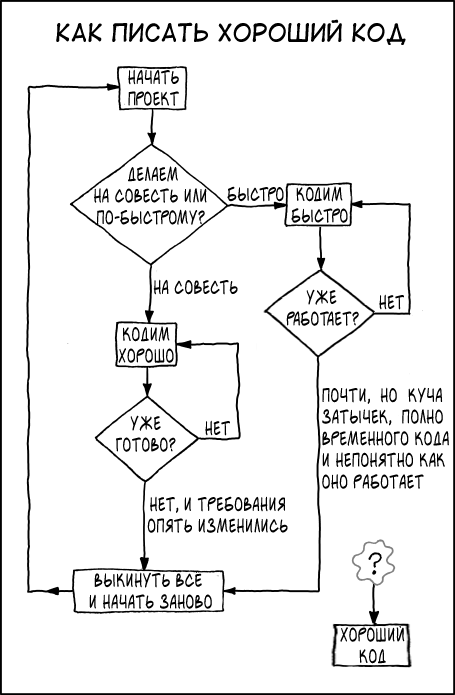
\includegraphics[scale=0.4]{img/2.png}
    \caption{Картинка о том, как писать хороший код :D}
\end{figure}

\clearpage

\nocite{*}

\printbibliography

\end{document}